% Chapter 7
\section*{Preface}
To find cheaper alternatives to the state-of-the-art, a wide range of solvents and current collectors were investigated while preparing cathodes and their performance was recorded. The purpose of this chapter was to test new current collectors (CCs) and solvents, and see if they were suitable for the non-aqueous aluminium battery system. Since the solvent and current collectors do not play an active role in storing charge in a battery, the capacity values obtained from these batteries was not a major concern. 
\newpage

\chapter{Impact of solvents and current collectors on rechargeable AIBs} % Main chapter title
\label{chap7} % For referencing the chapter elsewhere, use \ref{Chapter1} 

\section{Theory and background}

Battery electrodes are manufactured by casting a slurry onto a current collector (CC), which is generally a metal foil. A cathode slurry generally contains the active material, conductive carbon, and a polymer binder dispersed in a solvent. Synergy between the different components of a slurry enhances the electrochemical property of the electrode by placing the electrode particles closer together and increasing the conductivity of the slurry \cite{zheng_cooperation_2012}.
However, in 2004 Seki \textit{et al.} showed that the role of one additive is controlled by the other. For example, combination of an insulating binder and an oxide active material, would decrease the overall conductivity of the slurry \cite{guy_novel_2006, seki_effect_2004}. Therefore, optimization of electrode compositions is essential for the fabrication of high-quality electrodes. The solvent plays an important role in determining the slurry quality. A good solvent should provide high dispersivity, avoid decomposition of electrolyte/ electrode material and improve the compatibility between a slurry and the electrolyte. It should also prevent agglomeration of the particulate materials as that would lead to a poorly flowing slurry. Ludwig and his group reported that a non-uniform coating results in an uneven weight distribution on the CC further deteriorating the battery performance \cite{ludwig_solvent-free_2016}. N-methyl pyrrolidinone (NMP) is the premium choice for a solvent in most of the battery systems. It is polar and its functional groups provide enhanced adhesion with binders, especially polyvinylidene fluoride (PVDF) (see Figure \ref{Figures/chap7fig:nmppvdf}). Solvent evaporation is necessary for cell fabrication. Since NMP is an expensive solvent and an environment pollutant, ideally an NMP recovery system must be in place during the drying process to recover the evaporated NMP. However, new coating techniques and different solvents are now being developed to make battery manufacturing more economical. \cite{liu_effective_2014,spreafico_pvdf_2014, liu_effects_2008, lee_effect_2010, wenzel_challenges_2015, lee_selection_2017, stein_non-aqueous_2016}. In 2007, Lee and his group replaced the NMP/PVDF couple by water/elastomers (styrene-butadiene rubber) in lithium batteries. However, it was observed that the electrodes were not compatible with water and the batteries failed to deliver desired energy densities \cite{lee_novel_2007, li_effects_2005}. \\
To find cheaper alternative to NMP, new solvents such as isopropyl alcohol (IPA), toluene, acetone, methanol, butanol, dimethylsulfoxide (DMSO), dimethylformamide (DMF), dimethylacetamide (DMA), and acetonitrile were used (listed in Table \ref{tab1}) for preparing cathode slurries for non-aqueous AIBs. 

\begin{figure}[tbh!]
\centering
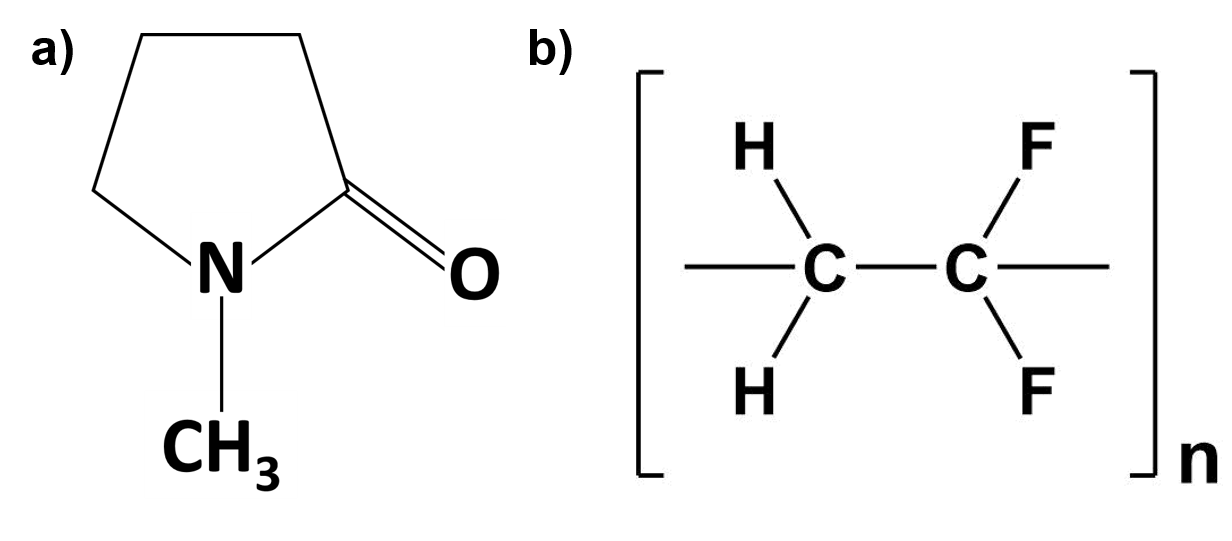
\includegraphics[width=0.5\textwidth]{Figures/chap7fig/nmppvdf}
\caption{Structure of a) N-methyl pyrrolidinone, NMP and b) polyvinylidene fluoride, PVDF.}
\label{Figures/chap7fig:nmppvdf}
\end{figure}

\begin{table}
\centering
\caption{List of solvents used for making cathode slurries.} \label{tab1}
\begin{threeparttable}
\begin{tabular}{|c|c|c|c|} 
\hline
\textbf{Solvent} & \textbf{Polarity} & \textbf{Boiling point} & \textbf{Price}\\
\textbf{} & \textbf{} & \textbf{($^{\circ}$C)} & \textbf{(\$ L$^{-1}$)}\\
\hline
Methanol & 0.76 & 64.7 & 51 \\ 
Butanol & 0.59 & 117.7 & 106 \\
Toluene & 0.09 & 110.6 & 106 \\
IPA & 0.55 & 82.5 & 133 \\
Acetone & 0.35 & 56 & 139 \\
DMF & 0.39 & 153 & 224 \\
DMSO & 0.44 & 189 & 230 \\
Acetonitrile & 0.35 & 82 & 236 \\
DMA & 0.35 & 165 & 241 \\
NMP & 0.35 & 202 & 277 \\
 \hline
\end{tabular}
\begin{tablenotes}
\item[*] Prices from Sigma Aldrich in NZD
\end{tablenotes}
\end{threeparttable}
\end{table}

\section{Experimental methods}

The first step was dissolving 18 mg of PVDF (6\% by weight) in 1.25 ml of anhydrous NMP. 27 mg (9\% by weight) of Super-P and 255 mg (85\% by weight) of the active material was then mixed the PVDF/NMP solution and stirred overnight. Once a homogeneous slurry was obtained, electrode laminates were prepared by casting the slurries onto a metal foil using the \enquote{doctor blading} technique. Each electrode had approximately the same loading of active material (around 5-6 mg cm$^{-2}$) to eliminate the thickness effect on the electrochemical performance of the electrode. After coating the foils, the laminates were dried at 80$^{\circ}$C for two hours and then at 120$^{\circ}$C for 12 hours under vacuum to evaporate the solvent. 
\section{Results and discussion}
Preliminary tests showed that DMSO, DMF, DMA, and NMP, when mixed with PVDF, resulted in clear solutions, while ethanol, isopropanol, toluene, acetone, methanol and butanol failed in dissolving the binder. The boiling point of the solvents also played an important role. Cathodes that used solvents having low boiling points such as acetone, ethanol, methanol isopropanol and acetonitrile, developed cracks on their surface due to high evaporation rates making them unusable. \\
Slurries that used DMSO, DMF, DMA, NMP, butanol and toluene as solvents yielded crack-free coatings. Consequently, they were used for electrochemical tests. The cathodes were tested via galvanostatic charge/discharge cycles and the results are displayed in Figure \ref{Figures/chap7fig:hBNsolventCDC}. Same active material (new h-BN) was used for all the cells to avoid discrepancies. DMSO-based cathodes displayed very low capacities although the cell maintained high CEs (>100\%) shown in Figure \ref{Figures/chap7fig:hBNsolventCDC} a and \ref{Figures/chap7fig:hBNsolventCE} a.  Figure \ref{Figures/chap7fig:hBNsolventCDC} b shows that the capacity of DMA based cathode was highest in its first cycle. Coulombic efficiencies of the cell, shown in Figure \ref{Figures/chap7fig:hBNsolventCE} b was also >100\% throughout. CE>100\% usually suggests side reactions and/ or cathode pulverisation as mentioned in previous chapters. Cathodes that used DMF as a solvent exhibited a CE of $\sim$99\% with capacity as low as 5 mAh g$^{-1}$ after 100 cycles. Unfortunately, the capacity retention for all the above- mentioned solvents was poor. NMP displayed a stable performance, shown in Figure \ref{Figures/chap7fig:hBNsolventCDC} d and \ref{Figures/chap7fig:hBNsolventCE} d. The cell maintained its capacity at 15 mAh g$^{-1}$ after 50 cycles with CE of $\sim$90\%. 

\begin{figure}[tbh!]
\centering
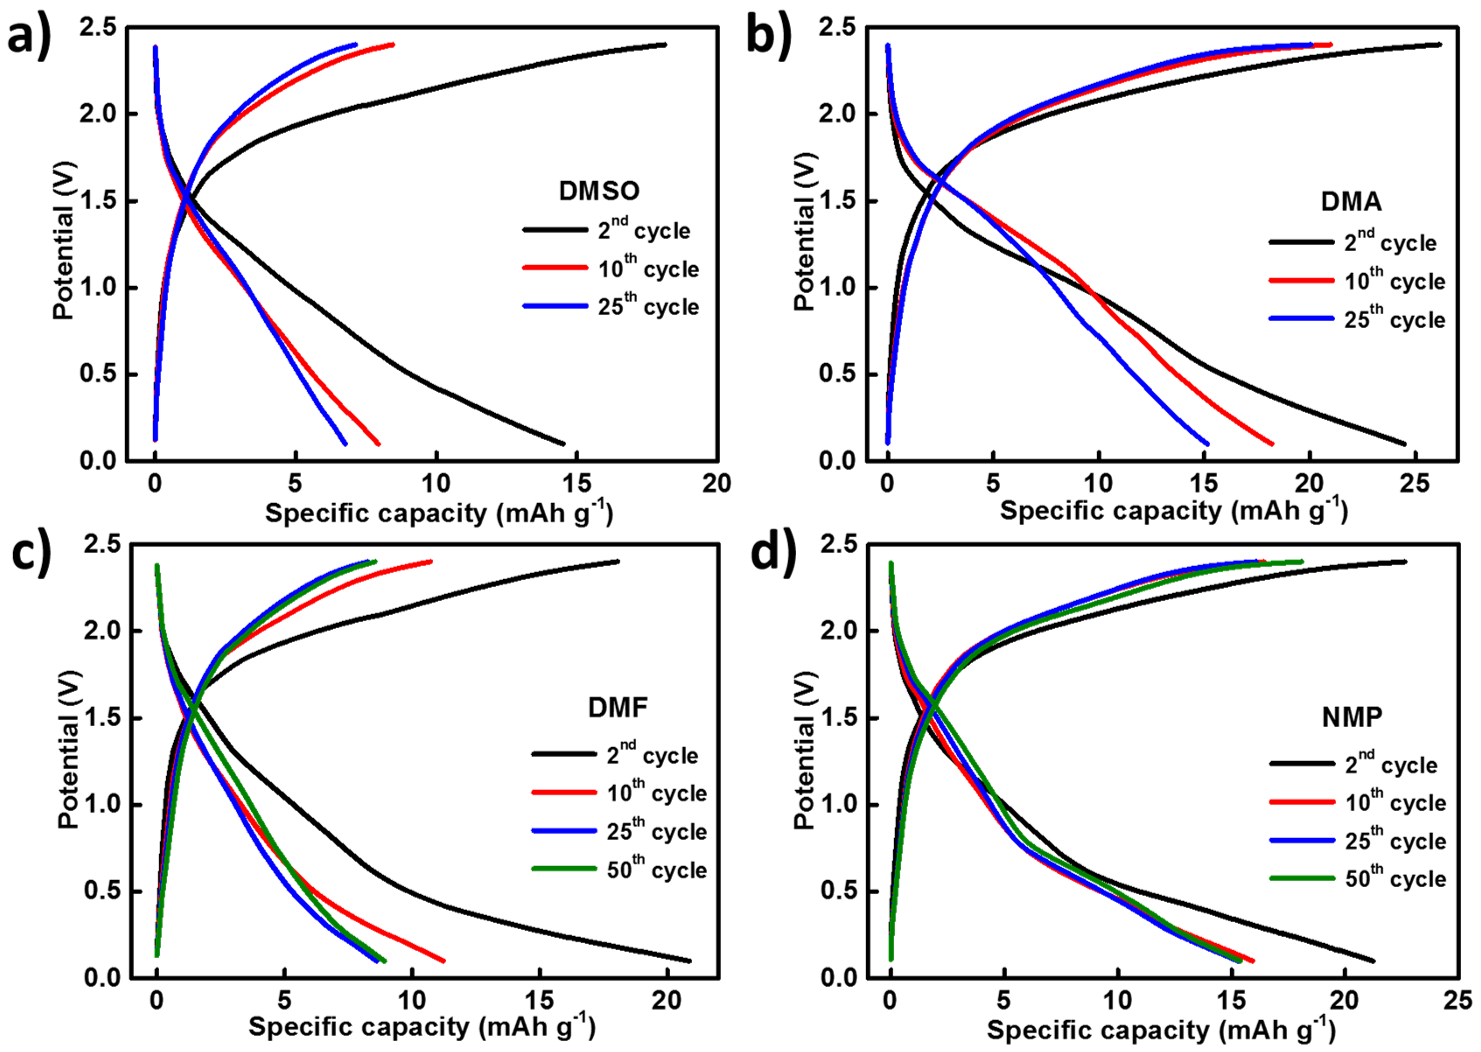
\includegraphics[width=\textwidth]{Figures/chap7fig/hBNsolventCDC}
\caption{Galvanostatic charge and discharge curves of aluminium-ion cells using different solvents, a) DMSO, b) DMA, c) DMF and d) NMP.}
\label{Figures/chap7fig:hBNsolventCDC}
\end{figure}

\begin{figure}[tbh!]
\centering
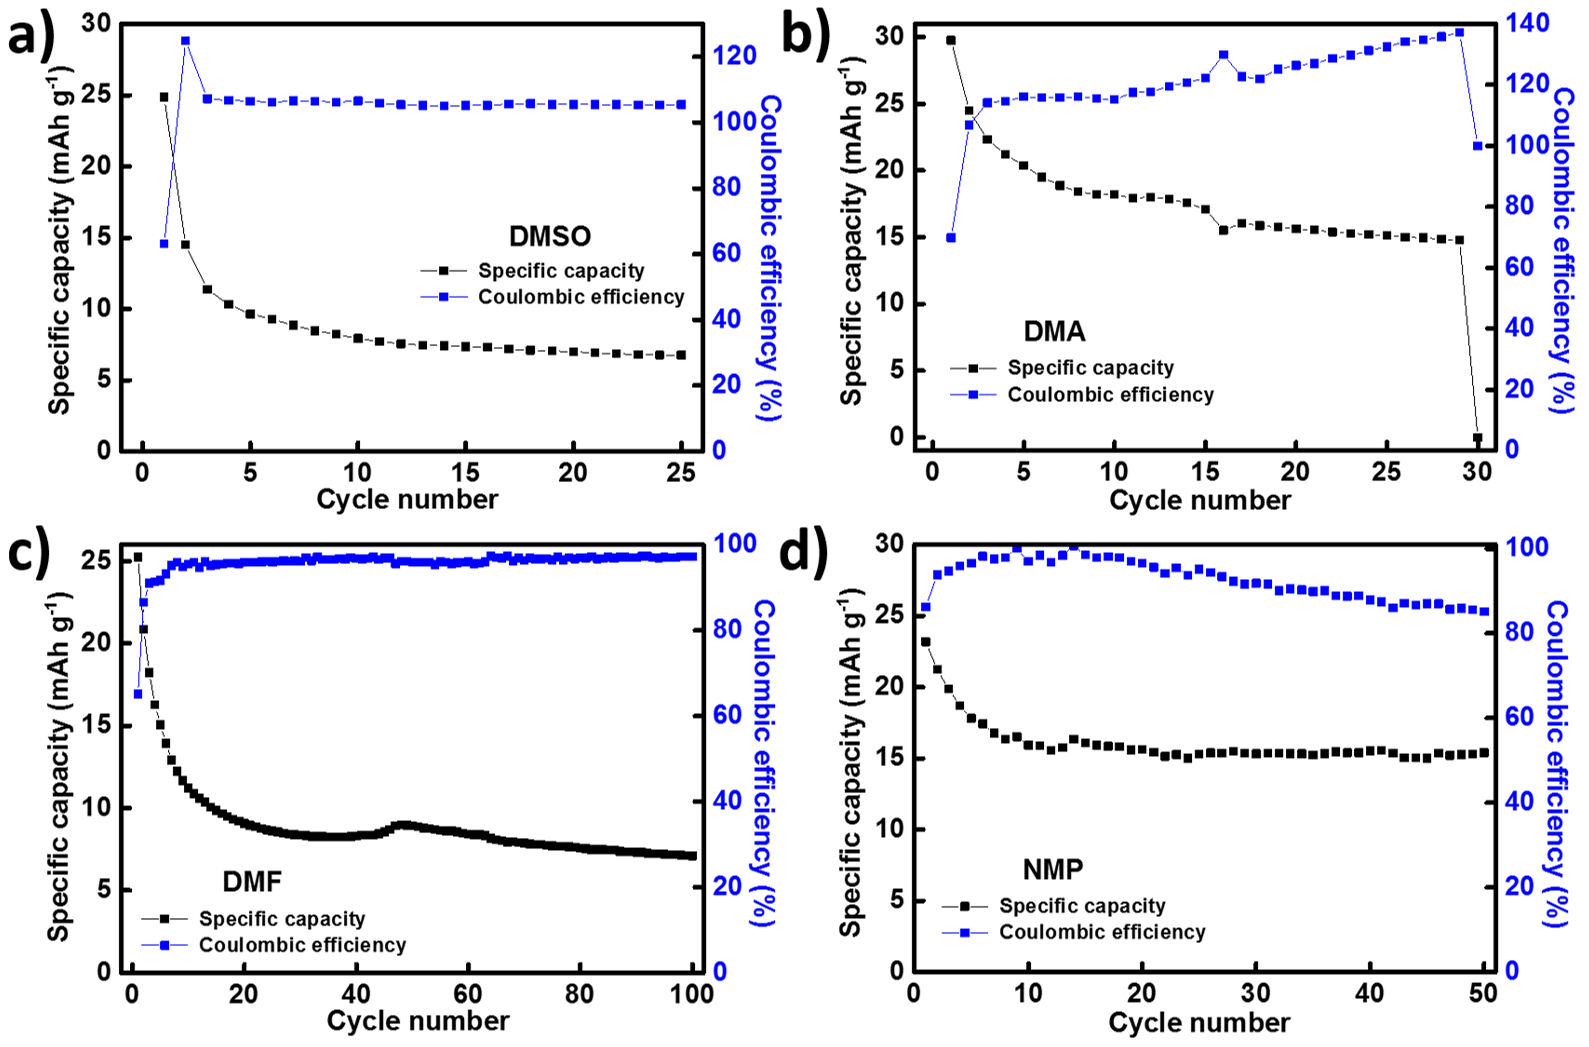
\includegraphics[width=\textwidth]{Figures/chap7fig/hBNsolventCE}
\caption{Performance of aluminium-ion cells using different solvents, a) DMSO, b) DMA, c) DMF and d) NMP.}
\label{Figures/chap7fig:hBNsolventCE}
\end{figure}

\begin{figure}[h!]
\centering
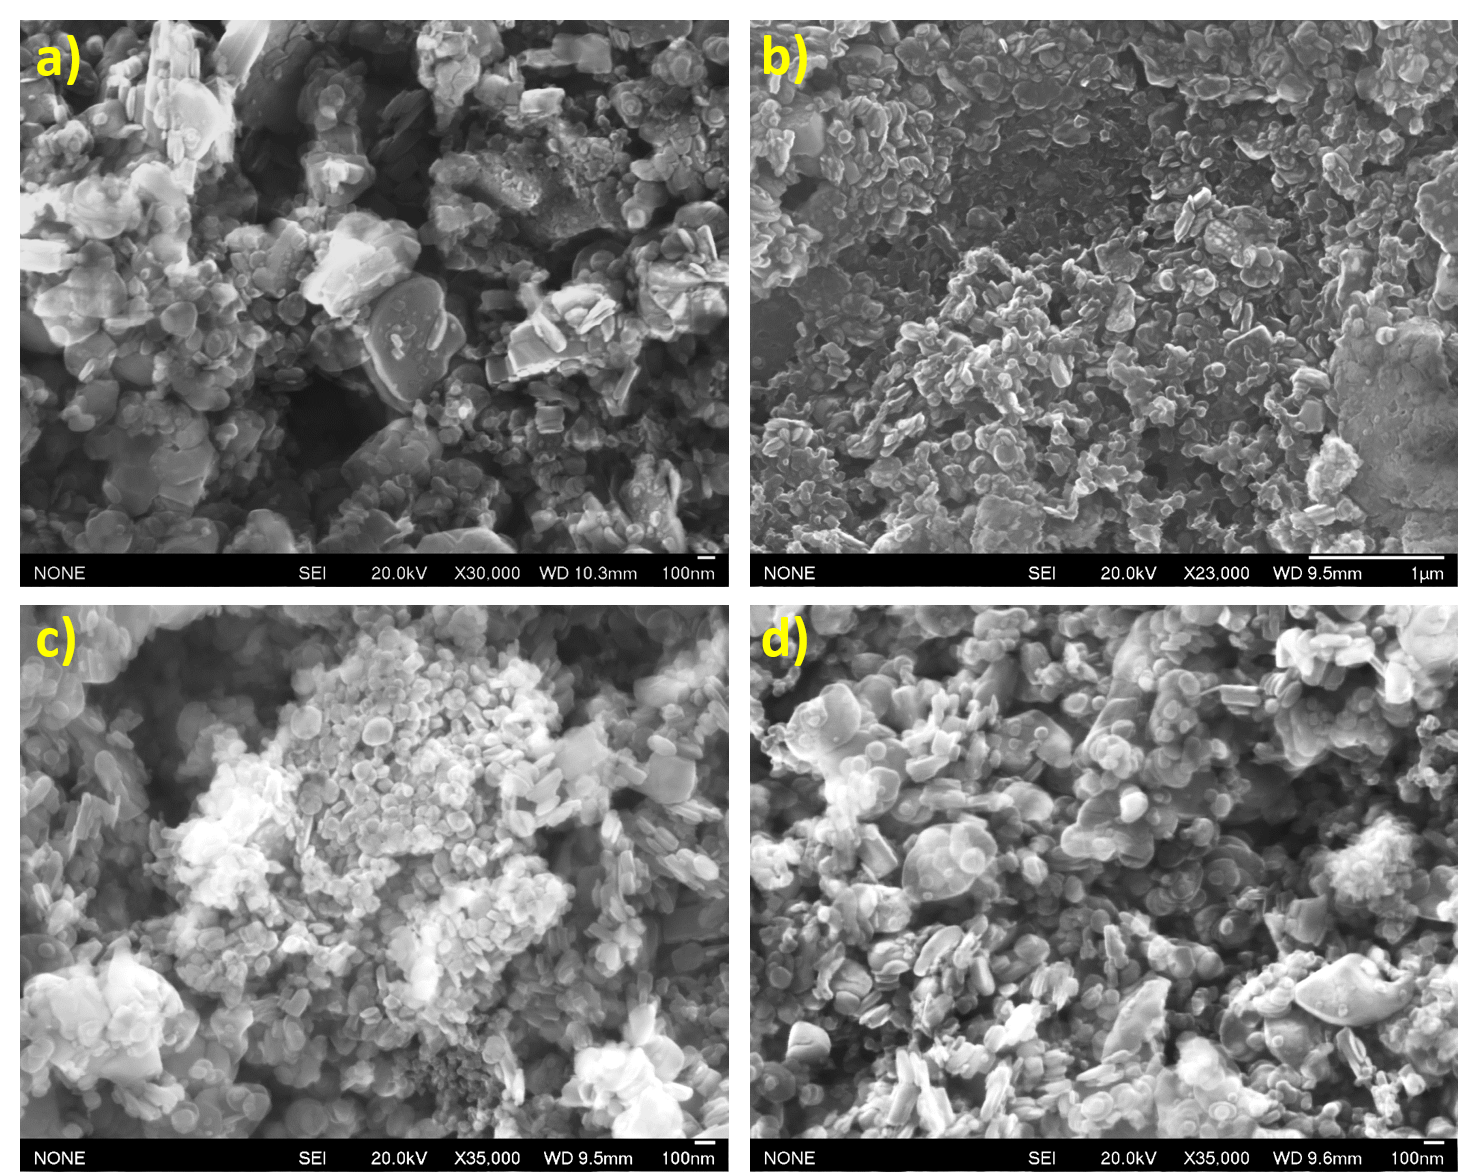
\includegraphics[width=\textwidth]{Figures/chap7fig/hBNsolventSEM}
\caption{Scanning electron microscopic images of pristine cathodes using a) DMSO, b) DMA, c) DMF and d) NMP as solvents.}
\label{Figures/chap7fig:hBNsolventSEM}
\end{figure}

Figure \ref{Figures/chap7fig:hBNsolventSEM} shows the SEM images of all the pristine cathodes. Cathodes that used DMSO and DMA showed prominent agglomeration of particles at few places, Figure \ref{Figures/chap7fig:hBNsolventSEM} a and b. In Figure \ref{Figures/chap7fig:hBNsolventCDC} c and d, DMF and NMP-based cathodes seemed to be immersed into a matrix of PVDF and Super-P additives. Despite having low capacity values, DMF was the only solvent that delivered a stable performance and was second-best to NMP. \\

\section{Current collectors}

\begin{table}
\centering
\begin{threeparttable}
\caption{List of materials used as CCs in increasing order of their market price.} \label{t2}
 \begin{tabular}{|c|c|c|c|} 
\hline
\textbf{Material} & \textbf{Thickness} & \textbf{Price per kg} & \textbf{Conductivity} \\
 & \textbf{(mm)} & \textbf{(NZD)} & {10$^{7}$} {$\Omega$}m$^{-1}$ \\
\hline
Steel & 0.1 & 1.0 & 0.6 \\ 
Carbon paper & <0.1 & 1.2 & 6.5 \\
Aluminium & 0.1 & 3.04 & 3.6 \\
Brass & 1 & 5.07 & 1.4 \\
Copper & 0.1 & 9.91 & 5.9 \\ 
Nickel foam & 1 & 17.93 & 1.4 \\
Molybdenum & 0.1 & 39.61 & 1.9 \\
\hline
\end{tabular}
\begin{tablenotes}
\item [*] Prices in NZD
\end{tablenotes}
\end{threeparttable}
\end{table}
A current collector (CC) is a conductive solid (generally a metal foil) connected to the electrode. The primary role of a CC is to provide support to the electrodes (cathode and/or anode), and collect the accumulated electrical energy from the electrode. A good connection between the active material and the metal foil is established only after a slow drying process which evaporates the solvent and binds it to the CC. Many metal foils have been used as CCs in LIBs, such as nickel, copper, aluminium and steel. LIBs use two different metal foils for each of its electrode. Copper is used as the CC on the anode side, while aluminium is used on the cathode side. Aluminium cannot be used as a CC on the cathode side in AIBs because any contact between the active material and the anode could short the circuit. Generally, during an internal short circuit of a battery, the two electrode materials connect electronically, giving rise to high local current densities. This can increase the temperature inside the cell due to the high power dissipation in the circuit. A CC should allow a stable flow of electrons, and should be ionically insulated. Table \ref{t2} lists all the metal foils that were used as CCs in this chapter for non-aqueous AIBs. Nickel foil starts oxidising at 1.1 V vs. Al/\ce{Al^3+} resulting in an \lq infinite\rq\ charging. This phenomenon was observed in a few cells in the beginning of the PhD project until it was replaced by molybdenum foil. The infinite charging of the cell using a nickel current collector is displayed in Figure \ref{Figures/chap7fig:nickel}. 
\begin{figure}[tbh!]
\centering
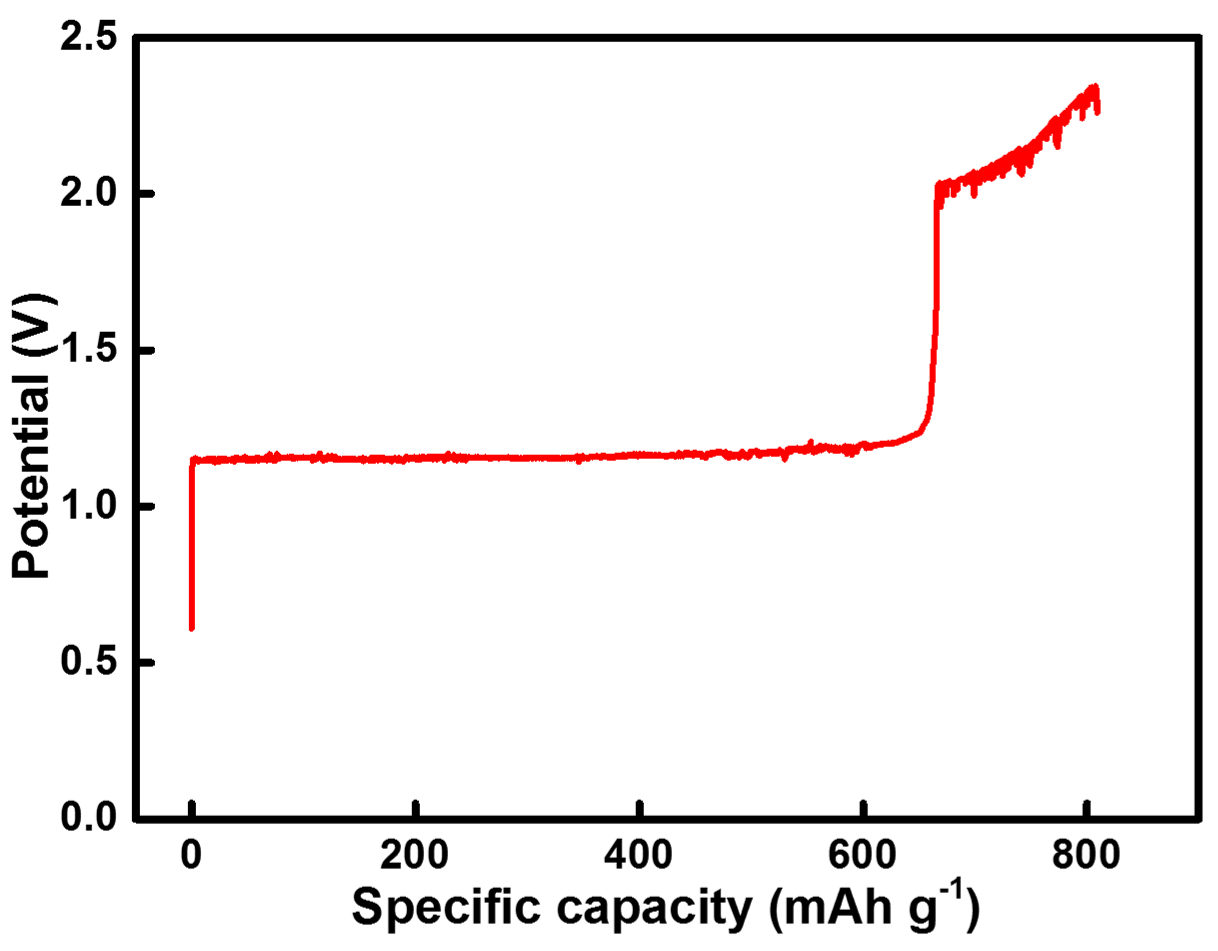
\includegraphics[width=\textwidth]{Figures/chap7fig/nickel}
\caption{\lq Infinite\rq\ charging taking place in the first cycle of an Al/\ce{MoS2} cell that use nickel as the current collector at a current rate of 50 mA g$^{-1}$.}
\label{Figures/chap7fig:nickel}
\end{figure}

Also, steel underwent a vigorous reaction with the \ce{AlCl3}/EMImCl electrolyte and formed undesirable products, shown in Figure \ref{Figures/chap7fig:steeleffect}, and the cells became inactive. A new CC was needed that would remain stable within the electrochemical window of the \ce{AlCl3}/EMImCl electrolyte. Molybdenum foil was also tested as a current collector. A cell was assembled using an uncoated Mo foil as the cathode, Al foil as the anode and \ce{AlCl3}/EMImCl as the electrolyte. The results obtained from the blank cell are displayed in Figure \ref{Figures/chap7fig:blankmo}. In 2019, Munoztorrero \textit{et al.} confirmed that molybdenum was indeed the best CC for non-aqueous AIBs. They tested molybdenum (Mo), tungsten (W) and tantelum (Ta) and it turned out that Mo was the least expensive of all metals after comparing the purchase cost per cycle \cite{munoztorrero_unexpected_2019}. The cost analysis performed by his group is shown in Figure \ref{Figures/chap7fig:goodmo}.
\begin{figure}[tbh!]
\centering
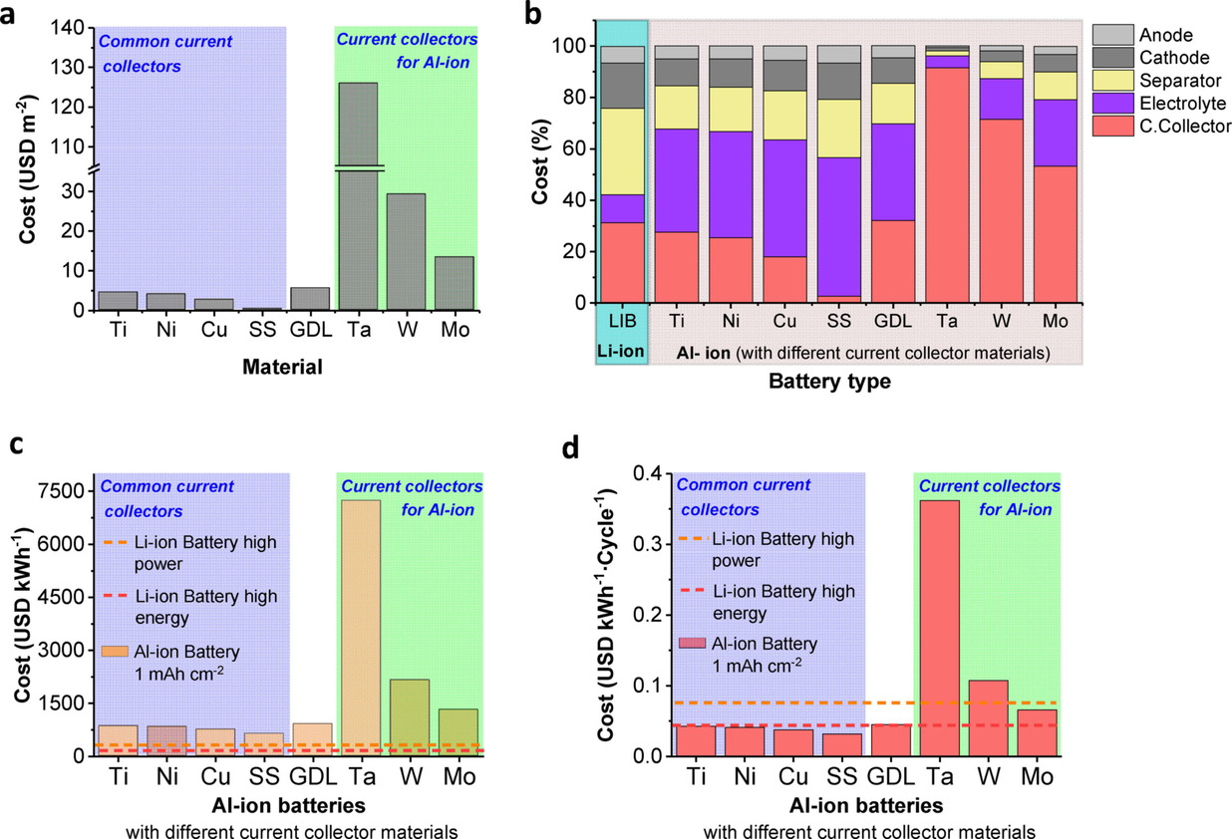
\includegraphics[width=\textwidth]{Figures/chap7fig/goodmo}
\caption{Cost (USD m$^{-2}$) of different current collector materials (thickness=50 $\mu$m). b) Contribution of each component to the purchase cost of LIB and AIBs using different current collector materials (areal capacity of 1 mAh cm$^{-2}$ for both Li and AIBs). c) Purchase cost (USD kWh$^{-1}$) and d) Purchase cost per cycle (USD kWh$^{-1}$ per cycle) of AIBs using different current collectors using state-of-the-art areal capacity of 1 mAh cm 2 and high-power LIB (areal capacity=1 mAh cm$^{-2}$) and high-energy LIB (areal capacity = 3 mAh cm$^{-2}$). }
\label{Figures/chap7fig:goodmo}
\end{figure}

\begin{figure}[tbh!]
\centering
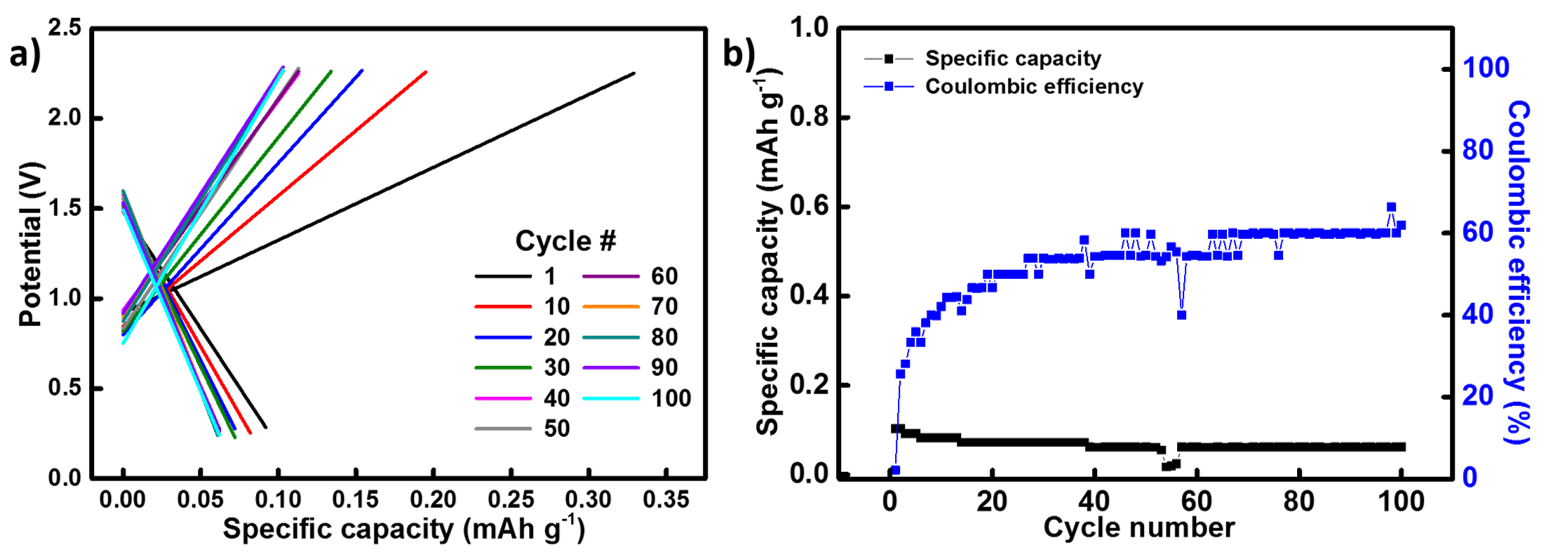
\includegraphics[width=\textwidth]{Figures/chap7fig/blankmo}
\caption{a) Charge/ discharge curves for Al/ molybdenum cell for 100 cycles. The cell displayed specific capacity at <0.10 mAh g$^{-1}$. b) Long-term cell stability test at a current rate of 50 mA g$^{-1}$ displaying its specific capacities during discharge and coulombic efficiencies for 100 cycles.}
\label{Figures/chap7fig:blankmo}
\end{figure}

\subsection{Results and discussion}
The performances of cells using different CCs is shown in Figure \ref{Figures/chap7fig:hBNCCCDC}. The cells became inactive when steel, nickel, copper, and brass foils were used as CCs as shown in Figure \ref{Figures/chap7fig:hBNCCCDC} a. Corrosion of these metals in the presence of \ce{AlCl3} might have resulted in the inactivity of the cells. In 2010, Tseng \textit{et al.} showed that steel starts corroding in presence of \ce{AlCl3}/EmImCl; Figure \ref{Figures/chap7fig:steeleffect} displays the effect of steel (present in the coin cell casings) on the EMImCl/\ce{AlCl3} electrolyte \cite{reed_roles_2013, tseng_corrosion_2010}. The reaction that takes place between (chromium present in steel) and the chloroaluminates anions is given below in Equation \ref{crsteel}.
\begin{equation} \label{crsteel}
4\ce{AlCl4- + Cr <=> 2Al2Cl7- + CrCl2 + 2e-} 
\end{equation}
Carbon as a CC recorded the highest discharge capacity at 82 mAh g$^{-1}$ (in green), which decreased to 70 mAh g$^{-1}$ after 25 cycles as shown in Figure \ref{Figures/chap7fig:hBNCCCDC} b. The charge/ discharge curves and the resulting capacity from the AIB using carbon paper as the CC were exceptionally similar to that of an Al/graphite cell (Figure \ref{Figures/chap7fig:hBNCCCDC} b inset). It was hence concluded that the active material had become dormant in this cell and graphitic carbon paper acted as the active material, successfully intercalating the \ce{AlCl4-} ions during charge and displaying a capacity of 70 mAh g$^{-1}$. Thus carbon paper was unsuitable as a freestanding CC. 
%The battery performance results are shown in figure 6. It can be seen that the charging behaviour of brass, copper and aluminium have a similar tendency. Starting from different voltages, charging the system does not result in an actual increase in voltage, thus charge built-up as desired. As shown in figure 6 a), brass, copper and aluminium tend to reach a specific equilibrium voltage regardless of the energy provided to the system. Energy consumption without any charging indicates other processes being present consuming the provided energy. It is assumed that the energy consumed is used to disintegrate the substrate material. Ideally, the substrate is not in direct contact with the electrolyte. In reality however there will always be some sort of contact area present. The Al atoms in the aluminium and eventually the iron or chromium atoms present in the brass and copper are resulting in the disintegration of the substrates as such. As a reference how a single charging/discharging cycle should appear, figure 6 b)	shows a complete cycle for a BN RAB using a molybdenum substrate. Here the desired charge built-up can be observed until reaching the cut-off limit of 2.4V and the following discharging can be observed. A very unique charging behaviour could be observed for carbon coated aluminium as a substrate for the hBN slurry as shown in figure 6 c). A mixture of fast charging and abrupt rapid discharging can be observed. Knowing the tendency of the aluminium shown in figure 6 a) to completely discharge to the cutoff voltage of 0.1, it can be assumed that the rapid discharging behaviour results from the underlying aluminium. As discussed in section 2, carbon based RAB have been shown to work well and achieve high charging rates. Therefore it is assumed that the charging phases are either caused by the BN cathode material or by the underlying carbon coating. Even though the just discussed tested alternatives did not succeed in charging at all, Ni foam and Carbon paper did successfully charge and discharge. The corresponding capacities are shown in figure 6 d). The fact that the capacity of the battery with Ni foam as substrate is noticeable lower is caused by the fact that nickel oxidises at voltages exceeding 0.9 V. This relatively low cutoff voltage is one reason why the capacity is rather low. It can be noticed that carbon paper as a substrate has a very high capacity. Comparing the achieved result however with results previously achieved by researchers of the VUW using carbon paper only, showed that that the overall performances are very much alike. This leads to the conclusion, that contrary to the desired hBN, mainly the carbon paper participated in the intercalation/deintercalation process. Therefore it is not a suitable substrate candidate for the specific use in the hBN based batteries due to the ions preferred affinity towards the carbon paper rather than to the hBN cathode material.
\begin{figure}[tbh!]
\centering
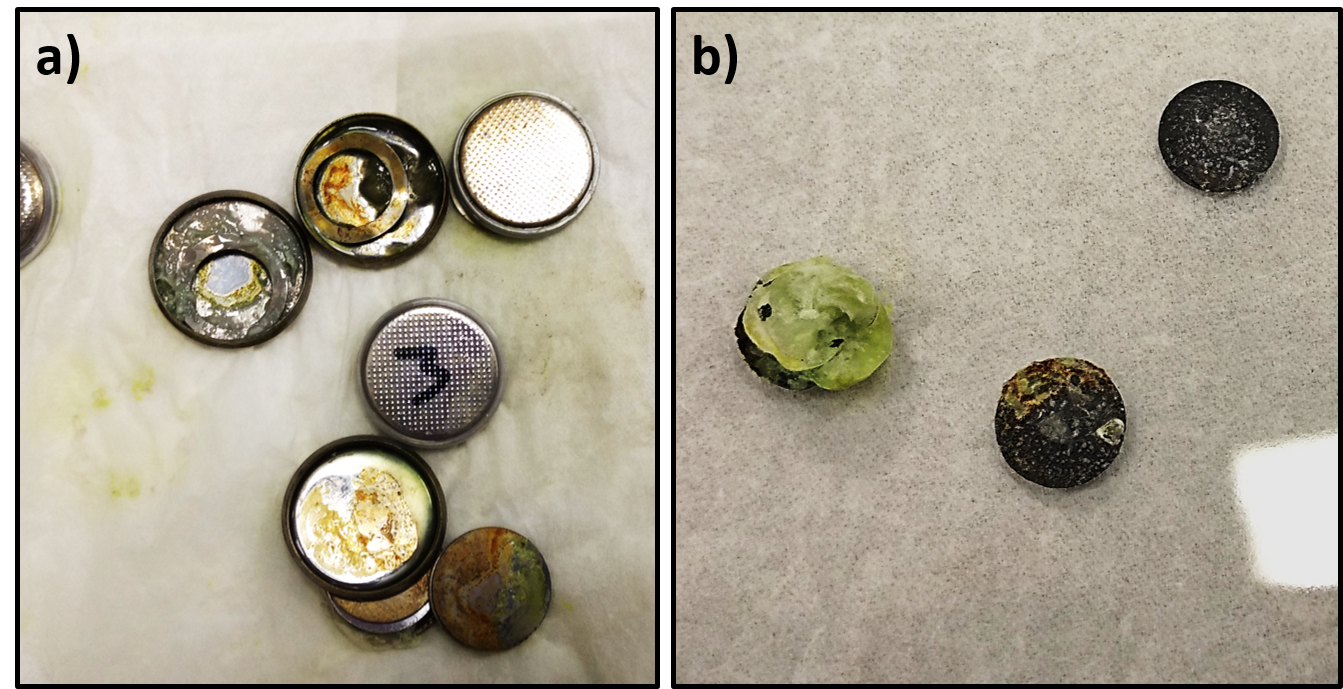
\includegraphics[width=\textwidth]{Figures/chap7fig/steeleffect}
\caption{Chromium present in stainless steel reacts with \ce{AlCl4-} and oxidises to form chromium chloride, which then diffuse to the aluminium anode where they are deposited during discharge. The reactions prevent the anode from further reactions and the cell becomes inactive.}
\label{Figures/chap7fig:steeleffect}
\end{figure}
\begin{figure}[tbh!]
\centering
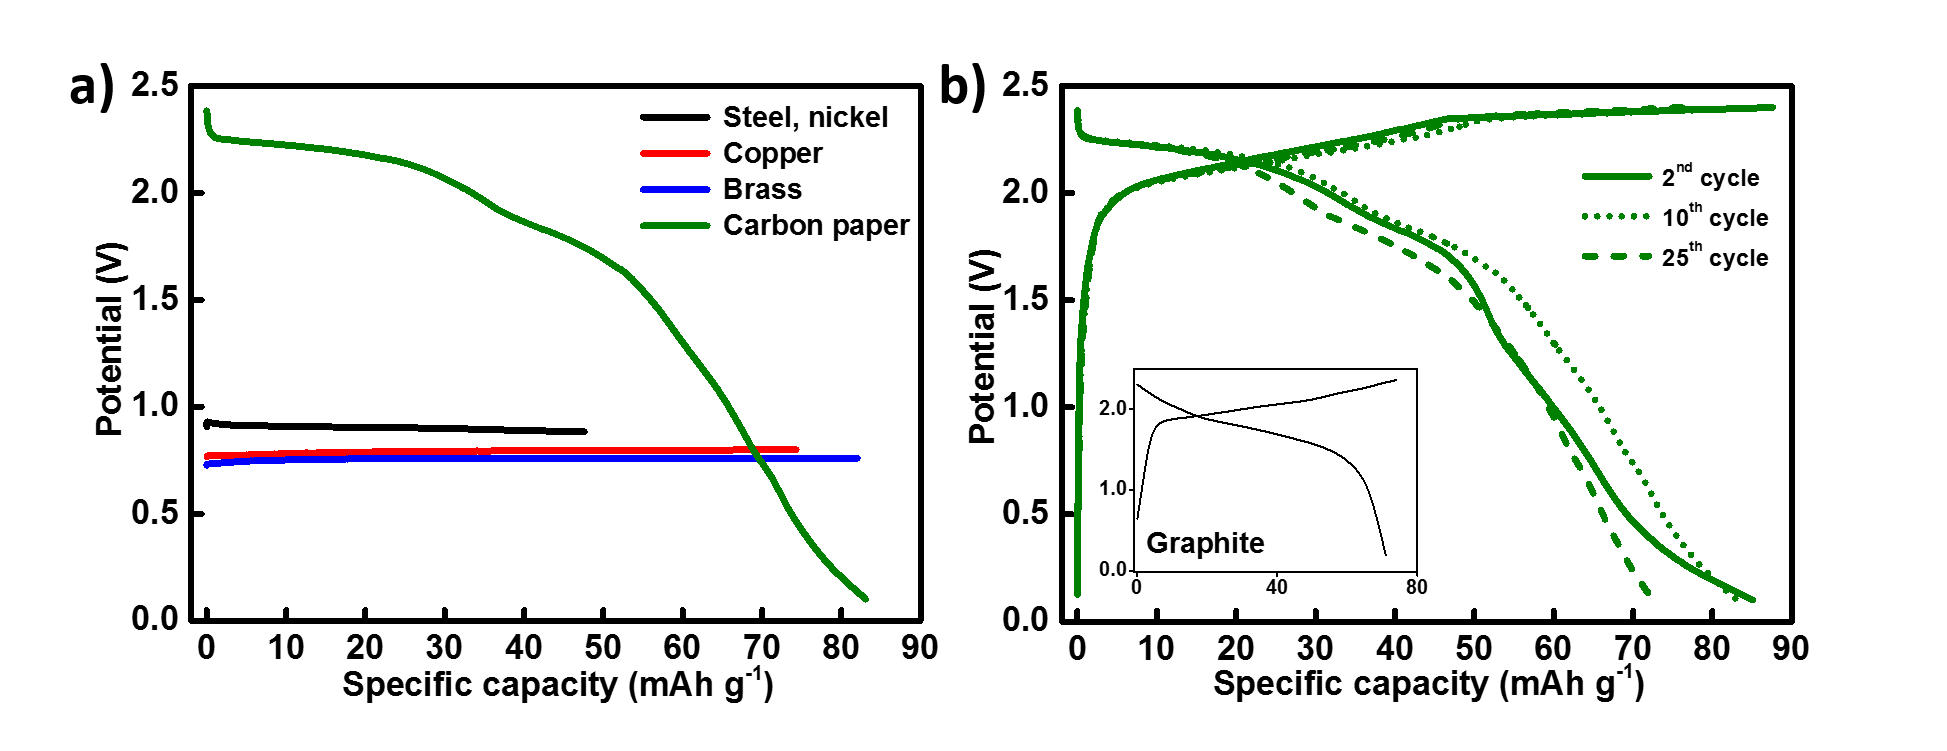
\includegraphics[width=\textwidth]{Figures/chap7fig/hBNCCCDC}
\caption{Galvanostatic cycles using hBN as the active material with a) steel and nickel foils (black), copper sheet (red), brass sheet (blue) and carbon paper (green) as CCs in a two-electrode setup at a current rate of 40 mA g$^{-1}$. b) Performance of Al/h-BN cell using carbon paper as the CC which showed graphite dominating as active material (inset: charge/discharge curve of an Al/graphite cell).}
\label{Figures/chap7fig:hBNCCCDC}
\end{figure}

\section{Summary}
Replacing NMP with a cheaper solvent would be beneficial when commercialising AIBs. However, no solvent tested in this chapter proved to be as efficient as NMP in the experiments conducted. However, 3-D carbon-based materials might make an interesting option as a CC in AIBs. In 2012, Ruoff \textit{et al.} used graphene foam as a CC for the first time \cite{ji_ultrathin_2012}. A 3-D CC provides a dense interconnected structure that can rapidly transport /diffuse ions, and improves the conductivity of the material. CCs with a large pore volume that accommodate expansion of active material would also prevent cathode pulverisation. Many different materials can be incorporated into their 3D structures, which allows them to be a free-standing material. Thus, one can explore further and find a suitable CC for non-aqueous AIBs.
